\documentclass[11pt]{article}

\usepackage{bridges}
\usepackage{graphicx} %% For including pretty pictures
\usepackage{url}      %% For formatting URLs.
\usepackage{amssymb}  %% for the square

\title{\textbf{Animation of Object-Oriented Program Execution}}

\author{
 	Peter Boothe\\
	Mathematics and Computer Science Department \\
	Manhattan College \\
	\url{peter.boothe@manhattan.edu}\\
        \\
 	Sandro Badame \\
	Computer Science Department \\
	University of Illinois, Urbana-Champaign \\
	\url{sandro@sbcoded.com}
}

\date{}

\bibliographystyle{plain}

%% Set the indentation at the start of paragraphs.
\setlength{\parindent}{0.3in}

%% Set the spacing between paragraphs.  The guidelines don't specify
%% that there should be a space, but I find paragraphs hard to read
%% without it.  I'm inserting a small space that you may choose to
%% modify.
\setlength{\parskip}{.75ex}

\begin{document}
\maketitle

%% Make sure not to include a page number on the first page.
\thispagestyle{empty}

\begin{abstract}

We describe a new system which animates the changing call stack and
object-reference graph of an object-oriented program that has not (necessarily)
been designed to be visualized.  We have sought to make the drawings and
animations produced by our system be beautiful in an effort to show
non-programmers what beauty and elegance might mean in the context of source
code.  Our animation system uses a new graph layout algorithm which produces
high-quality layouts in which many data structures naturally ``look right''.

\end{abstract}

\section{Animating the Execution of a Program}

In the past computer programs that produced artistic output have been exhibited
in art galleries next to the creations that they rendered. Often, the
program itself has been considered a work of art in its own right.
 Unfortunately, these efforts have never caught on.  This is in part
because the beauty of a computer program lies not in its source code, but in
the unfolding of its execution.

To an experienced reader, source code can be quite elegant and beautiful, but
it is completely inaccessible to the non-programmer.  This inaccessibility is
because in order to see the elegance of a program, the viewer is forced to
``play computer'' in their head to imagine the execution of the program.  If we
want to show people that computer programs can be beautiful, then we should use
an art form which can show program execution, that is, can display a system
which changes over time. Animation seems perfect for this as it is an art form
that allows drawings, much like programs, to change over time. 

In this paper, we debut a new system which animates the execution of Java
programs.  These Java programs need not be written with animation in mind, our
system will still display the execution of the program in a pleasing way.  If a
programmer would like, it is possible to tweak a program so that the
animation looks even better than the defaults, by changing the labels and
colors from their default values.

Previously, we developed a system\cite{boca} for the animation of the execution
of programs which can be represented as trees (roughly speaking, a subset of
Lisp), but that system required that the programs be written in a custom
dialect of Lisp, and, therefore, be written solely for the purpose of being
displayed.  Previous efforts at program animation have never had beauty as a
goal.  In all cases, the goals were more practical, and animations were for
comprehension, debugging, or for pedagogical help.  Although we hope our tool
might be useful in practical ways, the pursuit of beauty has proven to have its
own rewards.

\section{Our System: Memeograph}

Our system, Memeograph, works by running the ``work of art'' program (WOA) in a
separate Java Virtual Machine (JVM) that has been started in debug mode.
Usually debug mode is for more-traditional debuggers to connect to the JVM and
allow a programmer to debug their program. In our case, we use the debugger
connection to pause the WOA and retrieve from it all live objects, stack
frames, and object references.

When choosing what to visualize, one must choose both what to show, and also
what not to show.  In our case, we display the program stack, all stack frames,
all reachable objects, and all references between those items.  We do not
show the program source code, and we also ignore all the system threads of the
Java virtual machine (most of which are concerned with garbage collection).

We treat our non-ignored data as a graph, with objects and stack frames as
vertices, and object references as edges between vertices.  We then lay out
this graph in 3-dimensions according to our layout algorithm (next section).
Subsequently, we advance the virtual machine step by step, animating the
transition from layout to layout. What defines a step is configured through
Memeograph but it is most commonly defined as a point of execution directly
before a function of interest is called. Memeograph remembers past graphs,
and so can animate the execution of the WOA both forwards and backwards in
time.

\section{Layout of Program Memory}
\label{sec:layout}

Layout of general graphs is a hard problem with a rich literature surrounding
it (the 19th Graph Drawing symposium will be held this year --- Di~Battista et
al.\cite{gd}\ is a recommended introductory text), and the layout of graphs in
3-dimensions remains an area of active research.  In our system, we lay out the
objects using only the spanning-tree of the graph created from a breadth-first
search starting from the very top stack frame.  When laying out the program for
beauty, we note that there are multiple ways a program might be considered
elegant. 

Some programs achieve elegance through beautiful and intricate data structures
such as red-black trees or B+ trees or skip lists.  This is an elegance based
in using interesting or intricate data structures.  Even simple binary search
trees have proven to be quite nice-looking.  Other programs achieve elegance
through unique and surprising connections between software components --- a
very different sort of elegance in a very different domain.  This second kind
of elegance might be called elegance in software engineering.  We also note, for completeness, that there are more
senses in which a program might be called elegant --- including its runtime
efficiency or its brevity.  With Memeograph we attempt to deal with only two
kinds of program elegance, and leave the remaining senses for future work.

We would like our system to show off any elegance of the data structures and
software engineering in the WOA, so we have a heuristic which, literally,
attempts to make these two concerns orthogonal to one another.  Our heuristic
is that when a link goes between two vertices $(u,v)$, and $u$ and $v$ are
objects of the same type, or one is a child of the other, then $u$ and $v$ are
given the same $y$ coordinate, and instead $v$ is placed with a $z$ coordinate
behind $u$.  In all other cases, $u$ and $v$ are given the same $z$ coordinate,
and the $v$ is placed below $u$ via a greater $y$ component.  When like links
to like, the two vertices are placed at the same height, but at different
depths.  When like links to unlike, the two vertices are placed at the same
depth, but at different heights.

Data structures objects usually have large sub-parts where objects of the same
type link to one another, which means the vertices of an instantiated data
structure will tend to all have the same $y$ value.  This tendency makes the
$(x,y)$ plane the ``software engineering'' plane, and the $(x,z)$ plane the
``data structures'' plane.  An example layout in this style may be seen in
Figure~\ref{fig:basic}, which contains a program with almost no interesting
features in the software engineering plane. but does contain both a linked list
and a binary search tree drawn in the data structures plane.  

\begin{figure}
\begin{center}
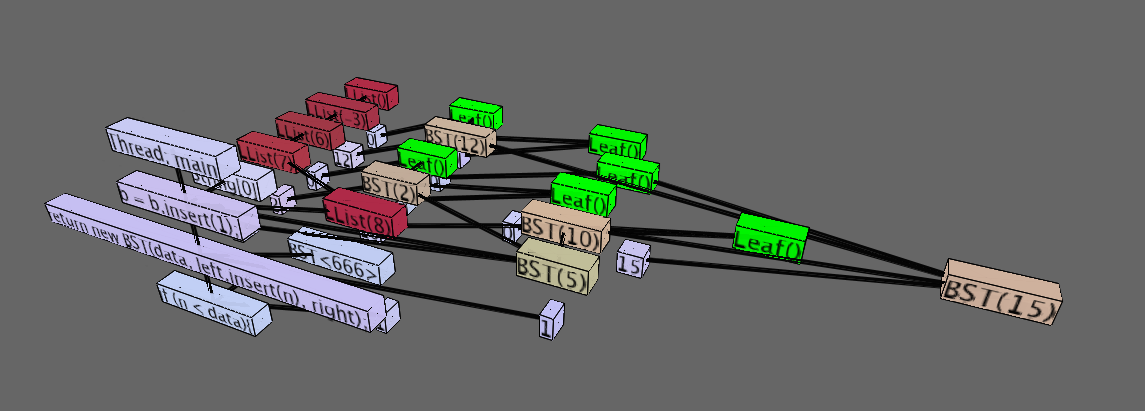
\includegraphics[width=5in]{figures/basic.png}
\end{center}
\caption{A program containing both a linked list (colored red) and a binary
search tree (internal nodes are brown, and the leaves are green).  This program
contains almost no interesting features in the software engineering plane, but
does manage to draw some fundamental data structures in the data structures
plane.}
\label{fig:basic}
\end{figure}

\begin{figure}
\begin{center}
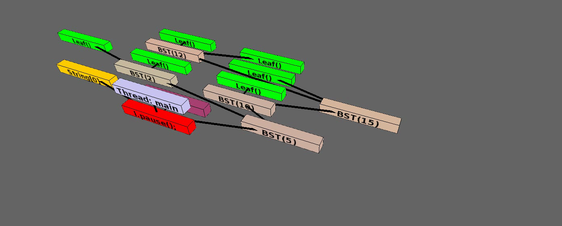
\includegraphics[width=1.5in]{figures/bar-010.png}
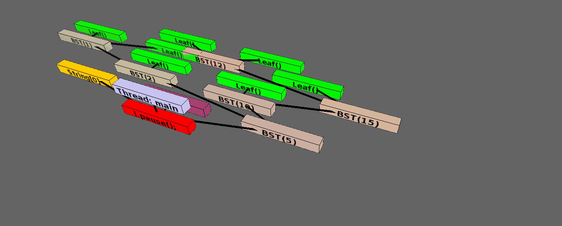
\includegraphics[width=1.5in]{figures/bar-012.png}
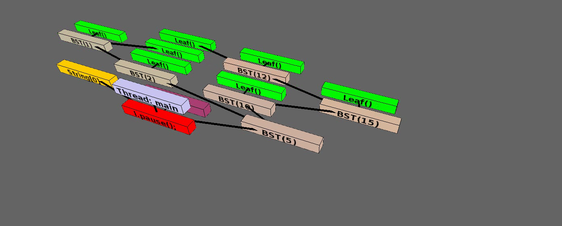
\includegraphics[width=1.5in]{figures/bar-014.png}
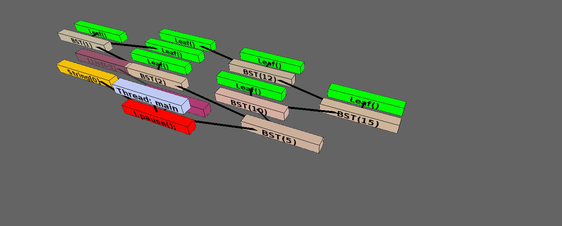
\includegraphics[width=1.5in]{figures/bar-016.png}
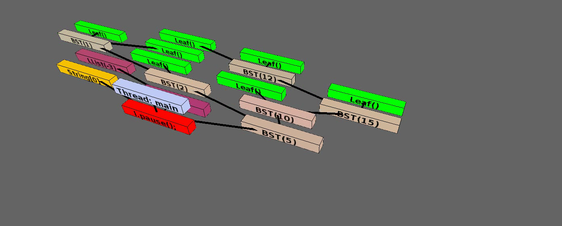
\includegraphics[width=1.5in]{figures/bar-018.png}
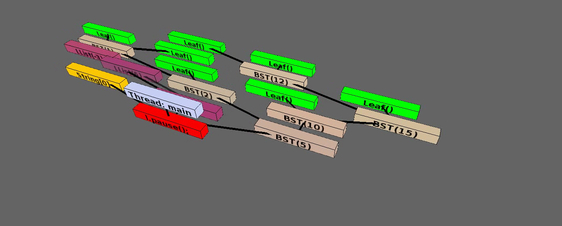
\includegraphics[width=1.5in]{figures/bar-022.png}
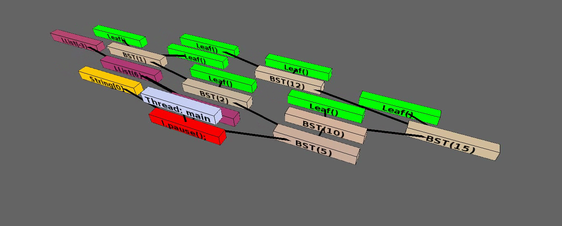
\includegraphics[width=1.5in]{figures/bar-024.png}
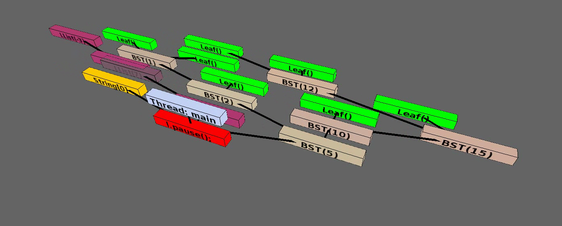
\includegraphics[width=1.5in]{figures/bar-026.png}
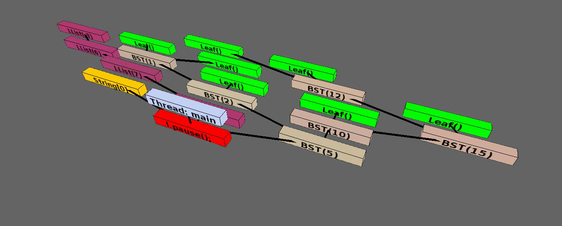
\includegraphics[width=1.5in]{figures/bar-028.png}
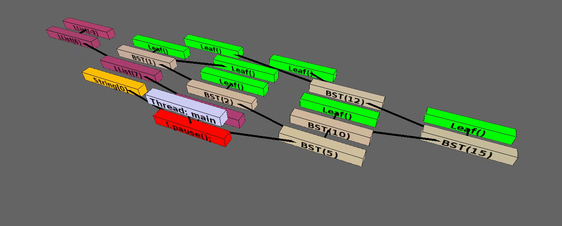
\includegraphics[width=1.5in]{figures/bar-030.png}
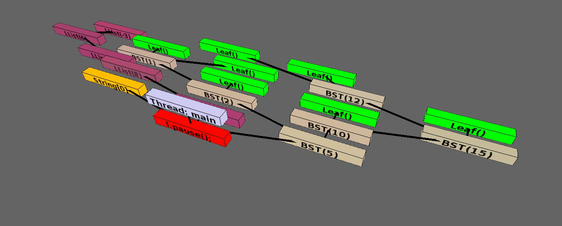
\includegraphics[width=1.5in]{figures/bar-032.png}
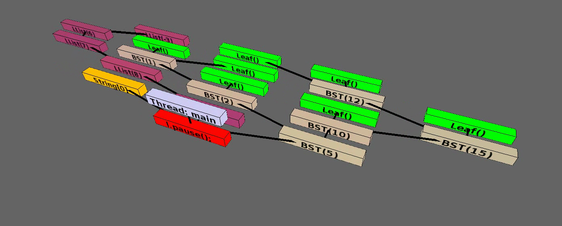
\includegraphics[width=1.5in]{figures/bar-034.png}
\end{center}
\caption{Frames from the animation of the last insertion into the BST and the prepending to the linked list resulting in Figure~\ref{fig:basic}.}
\end{figure}

When laying out trees, we have our choice of algorithms.  The most famous
algorithm for tree animation comes from Cohen et al.\cite{tamassia}, which
describes a geometrically inspired algorithm for 2-dimensional tree layout
(called the $\square$-algorithm), a set of allowed update operations for the
tree, and, for each operation, a smooth transition that allows the tree to be
smoothly animated through the transition.

Our layout algorithm, the cubic algorithm, is a straightforward extension of
their algorithm into the third dimension.  In an effort to strive for
generality, however, we do not limit the allowed transforms the tree might
undergo.  Instead, we take two successive trees, lay out each one, and then
identify the vertices the two trees have in common.  Vertices present in the
first tree, but not the second, are faded out in animation.  Vertices present
in the second tree, but not in the first, are faded in.  Vertices present in
both trees are gradually moved from their position in the first tree to their
position in the second tree.  Edges are faded in and out with the vertices to
which they are incident.

In this animation technique, we use the layout of each graph as ``key frames''
in our animation, and then produce the ``tween frames'' to move from one key
frame to the other.  Pleasantly, this mirrors how cartoons were often animated,
with the lead cartoonist creating the key frames, and supporting artists doing
the tween frames.  In Memeograph, our more-complicated layout algorithm
produces the key frames, and then simple linear interpolation produces the
tween frames.

The only remaining choice is when to make the key frames.  This is a
configurable option.  We allow the program user to specify what function calls
should generate a new tween frame.  As a promising default for new users, we
suggest generating a new frame every time {\tt PrintStream.println(String s)}
gets called, which will generate a new key frame every time the WOA prints a
message to standard out.

\section{Summary}

Visualizing software has never been done with beauty in mind, but programs can
be beautiful, and we should show that beauty to others.  Our system,
Memeograph\nocite{memeograph}, attempts to draw on the screen what was
previously only available to the original programmer: the intricate and
beautiful changing connection patterns of a running program.

\begin{figure}
\begin{center}
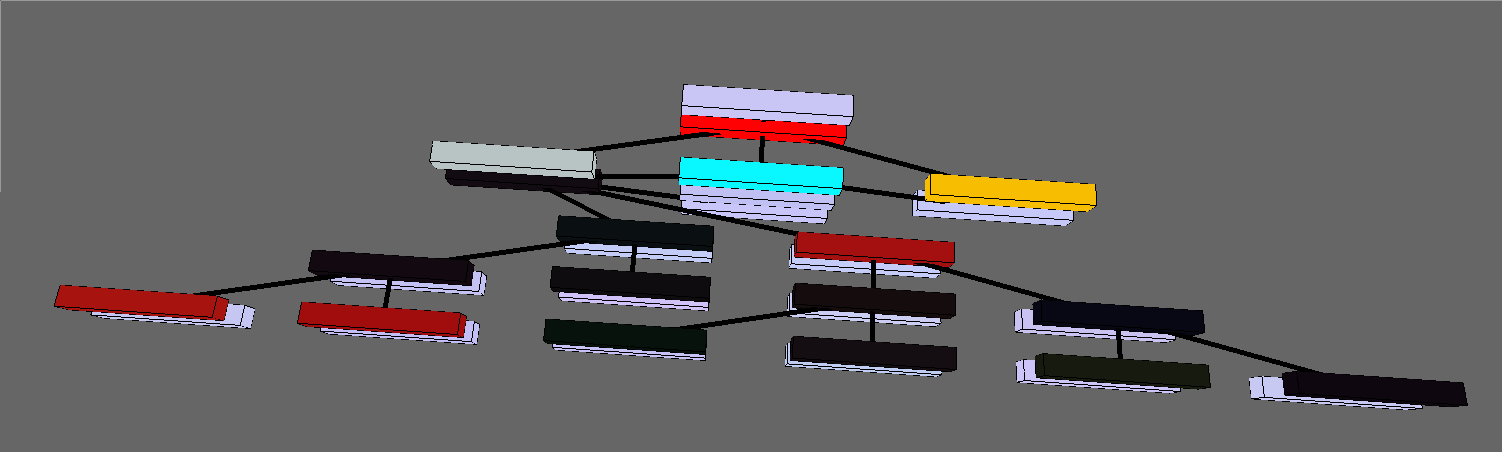
\includegraphics[width=5in]{figures/llrb.png}
\end{center}
\caption{A data-structure plane view after inserting the numbers 1 through 13
in order into a left-learing red-black tree.  Code taken from the original
paper\cite{llrb}, with two lines of code modified to make black nodes appear
black and red nodes appear red in our visualization.}
\end{figure}

In pursuing this goal, we ended up extending an existing graph layout
algorithm, as well as developing a heuristic that separates the drawing of the
program into the two kinds of elegance a program might contain: elegance in
software engineering (intricate connections between distinct components) and
elegance in data structures (intricate connections between like components).
These two kinds of elegance are subsequently drawn in distinct planes, so that
the viewer can choose the aspect on which to concentrate.

The generality of this method is one of its strengths.  The programmer need not
concern themselves with how their program looks, or, indeed, with any concern
for layout at all.  A program can be animated with absolutely no modification
by the original programmer.  It is possible to tweak the animation in order to
more clearly show certain effects, but our animation tool is able to treat any
Java program as a work of art.

\setlength{\baselineskip}{13pt} 
\bibliography{mybib}

\end{document}
